\documentclass[conference]{IEEEtran}
\IEEEoverridecommandlockouts
% The preceding line is only needed to identify funding in the first footnote. If that is unneeded, please comment it out.
\usepackage{cite}
\usepackage{amsmath,amssymb,amsfonts}
\usepackage{graphicx}
\usepackage{algorithm}
\usepackage{textcomp}
\usepackage{xcolor}
\usepackage{verbatim}
\usepackage{braket}
\usepackage{amsmath}
\usepackage{algorithm}
\usepackage{tabularx}
\usepackage{algpseudocode}
\usepackage{multirow}
\usepackage{algpseudocode}
\usepackage{physics} % For \ket{}
\usepackage{subcaption}

\usepackage{booktabs}
\usepackage{url}
%\usepackage[ruled,vlined]{algorithm2e}

\def\BibTeX{{\rm B\kern-.05em{\sc i\kern-.025em b}\kern-.08em
    T\kern-.1667em\lower.7ex\hbox{E}\kern-.125emX}}
\begin{document}

\title{Evaluating LLM-Generated Hardware for Quantum Circuit Simulation\\
%\thanks{We extend our gratitude to the National Science Foundation (NSF) for supporting this project under Award \#2512983.}
}

\author{
\IEEEauthorblockN{
Krishna Patel\textsuperscript{2,*},
Sumera Anjum\textsuperscript{2},
Spencer Buchanan\textsuperscript{1},
Xuechen Zhang\textsuperscript{3},
Yunhe Feng\textsuperscript{2},
and Xiaokun Yang\textsuperscript{1}}
\IEEEauthorblockA{
\textsuperscript{1}\textit{University of Houston--Clear Lake}, Houston, TX, USA \\
\textsuperscript{2}\textit{University of North Texas}, Denton, TX, USA \\
\textsuperscript{3}\textit{Kennesaw State University}, Kennesaw, GA, USA \\
\textsuperscript{*}REU participant}
}

\maketitle
\begin{abstract}
%State-vector simulation of an $n$-qubit circuit controls $2^n$ complex amplitudes, and FPGA accelerators built from a library of pipelined gate modules reduce its cost. Composing such a library for a new circuit is a hardware-design task. Large language models (LLMs) can write hardware description language, but prior work decides whether the output is correct against a testbench written for that design, an artifact that must itself be right. This paper presents a system that generates top-level SystemVerilog over a previously verified quantum gate library by preloading the library's non-derivable facts, such as exact port lists and a composition rulebook, into every prompt and retrieving one structurally similar worked example. Correctness is decided by simulating the generated design against a statevector computed directly from the Qiskit specification, so no reference RTL enters the verdict. 

This paper presents and evaluates a framework for LLM-assisted hardware generation for quantum circuit simulation using \texttt{gemini-3.5-flash}. The framework combines library interfaces, integration rules, a retrieved worked example, static linting, and bounded repair to translate \textit{Qiskit} circuits into \textit{SystemVerilog} hardware implementations. Evaluation covers 55 circuits spanning two-, three-, and five-qubit families, with generation prompts containing 3,688--4,026, 2,979--4,266, and 9,076--9,314 input tokens per circuit, respectively. Of the 55 generated implementations, 53 (96.4\%) produce state vectors that match the \textit{Qiskit}-derived references under the evaluated inputs and numerical tolerances. FPGA implementation results on the AMD Alveo U250 show maximum operating frequencies of 416--828~MHz and characterize resource utilization. In simulation, all ten generated designs with a reference match their reference's cycle latency exactly. \vspace{8pt}

%This paper presents a hierarchical framework that uses the \texttt{gemini-3.5-flash} large language model (LLM) to generate hardware for quantum circuit simulation. The framework integrates preverified and optimized quantum-gate building blocks, such as Hadamard and CNOT gates, to generate \textit{SystemVerilog} implementations of 55 circuits across the 2-, 3-, and 5-qubit families. Functional verification against reference state vectors produced using \textit{Qiskit} indicates that 53 of the 55 generated circuits yield matching results. Performance evaluation utilizing an AMD Alveo U250 Data Center Card demonstrates maximum operating frequencies ranging from 416 to 828 MHz for the 14 placed and routed designs. These results demonstrate the potential of LLM-assisted hierarchical hardware generation while emphasizing opportunities to improve the correctness and optimization of the generated designs.

%One failure is a library defect; the other is a generation error that passed its screened input and failed only when re-simulated from inputs covering every qubit exchange. The same verification exposed three defects in artifacts assumed correct---a reference implementation whose error is invisible to the input it is customarily driven from, a sign-extension bug in the gate library, and a handshake that asserts valid before its data settles. On one circuit the model routed a qubit exchange the hardware has no module for through three permutations, and exchange-sensitive inputs confirm the route.
\end{abstract}


\begin{IEEEkeywords}
LLM, Hardware Generation,
quantum circuit simulation, retrieval-augmented generation,
functional verification
\end{IEEEkeywords}

% =====================================================================
% I. INTRODUCTION
% =====================================================================
\section{Introduction}
\label{sec:intro}
Quantum circuit simulation is essential for validating quantum algorithms before execution on physical devices. However, state-vector simulation requires
processing $2^n$ complex amplitudes for an $n$-qubit circuit, leading to
exponential growth in computational cost that limits
simulation scalability and increases latency\cite{ali2026fpga,cicero2025simulation}.
Field-programmable gate array (FPGA) implementations offer opportunities
to accelerate simulation through custom amplitude encodings, deep
pipelines, and spatial parallelism. Prior work has demonstrated
nanosecond-scale simulation of small-scale quantum algorithms such as circuit cutting and QFT, using specialized classical hardware designs~\cite{isqed2026,hpdc26,TurnerICDM2025}.
However, the rules for composing hardware modules into complete designs are written manually for each circuit family. To lower
the hardware design barrier, this paper evaluates whether a large language model (LLM) can automate this composition step while maintaining performance comparable to that of manually composed designs.

Two challenges must be addressed before an LLM can perform this task~\cite{tran2025qea,gu2025precision,podobas2023q2logic}.
First, a gate library contains facts that cannot be inferred from the
circuit being implemented, which we refer to as \emph{non-derivable}
knowledge. Examples in the library used here include a module-numbering
scheme with gaps, ports removed during synthesis, and a native gate
orientation that reverses control and target. Second, verifying the correctness of
generated hardware is challenging. Existing benchmarks for
LLM-based hardware description language (HDL) generation, such as
\textit{VerilogEval}~\cite{verilogeval2023} and \textit{RTLLM}~\cite{rtllm2024}, score each design against an established testbench.
%Comparing a generated design structurally against a reference implementation is less costly but depends on the reference in the same way, and Section~\ref{subsec:structural} shows that such a comparison would certify as correct any generated design that reproduced a defect present in a reference implementation from this project.

To address the two challenges, this paper first measures results from a prompt-only study involving 661 generated designs, of which 372 passed simulation. The proposed system supplies this knowledge in every prompt, along with one retrieved worked example, and generates a top-level \textit{SystemVerilog} module that instantiates a pre-verified gate library~\cite{isqed2026,hpdc26}. Additionally, this paper simulates the generated designs against state vectors computed from the \textit{Qiskit} specification, so that no reference design is involved.

%Incorrect output amplitudes were the most frequent failure, followed by omitted permutation wrappers and the instantiation of modules that do not exist. The latter two classes arise from missing information, since a permutation wrapper is required by the hardware but does not appear in the logical circuit, and a module name cannot be deduced from the material the model is given.

%This paper presents a system that supplies this knowledge in every prompt, together with one retrieved worked example, and generates a top-level SystemVerilog module that instantiates the gate library. The correctness of each generated design is determined by simulating it against a statevector computed from the Qiskit specification, so that no reference design is involved and a circuit without a reference implementation is scored in the same way as one with a reference. Across three circuit families, 53 of the 55 evaluated circuits match their golden state. One of the two failures is attributable to a defect in the gate library. The other is a generation error that was not visible from the single basis input initially used for scoring and was detected only when the design was re-simulated from a set of inputs sensitive to every qubit exchange. Three further circuits fall outside this count. For one, no admissible test input exists; one exceeds the output length of the model; and the full QFT, although generated, is left unscored by the same input screen. This pass rate is not comparable with that of the prompt-only study, which used different circuits, three models, and a different prompt context. The evaluation also identified three defects in artifacts that had previously been assumed correct, of which two are functional and one concerns timing.

% ---- Contributions list ----
% Numbered 1) 2) 3) to match the companion paper's format.
Specifically, the main contributions of this work are as follows:
\begin{enumerate}
\item A hierarchical hardware generation framework that combines explicit library knowledge, a retrieved worked example, and automated lint-driven repair to generate top-level \textit{SystemVerilog} implementations for 2-, 3-, and 5-qubit circuit families. The assembled prompts contain 3,688--4,026, 2,979--4,266, and 9,076--9,314 input tokens per circuit, respectively.

\item A functional verification methodology that compares generated hardware outputs against golden state vectors computed directly from \textit{Qiskit} specifications, eliminating the need for reference \textit{Verilog} implementations and exposing errors that structural comparison can miss.

\item A prompt-only study of 661 generated hardware designs across varying circuit complexities, specification formats, prompt detail levels, and three models. The study demonstrates the importance of explicit hardware context, with simulation pass rates ranging from 29.2\% for sparse prompts to 88.2\% for full prompts.

\item A framework evaluation in which 53 of 55 generated implementations (96.4\%) match the golden state vectors under the evaluated inputs and numerical tolerances. FPGA implementation results for 14 designs on the AMD Alveo U250 show maximum operating frequencies of 416--828~MHz and characterize resource utilization. In simulation, all ten generated designs that have a reference match their reference's cycle latency exactly.

\item To support reproducibility and facilitate future research,  we make the project source code and benchmarking framework publicly available in an open-source GitHub repository~\cite{llm_hardware_github}.
\end{enumerate}


% =====================================================================
% II. RELATED WORK
% =====================================================================
\section{Related Work}
\label{sec:related}

\noindent\textbf{LLMs for HDL generation.} Benchmarks for LLM-generated \textit{Verilog},
including \textit{VerilogEval} and \textit{RTLLM}, determine correctness by simulating each
output against a testbench written for that
task~\cite{verilogeval2023,rtllm2024}. Subsequent systems incorporate
feedback from design tools. \textit{RTLFixer} repairs syntax errors by
combining compiler feedback with expert guidance retrieved at generation
time~\cite{rtlfixer2024}, while \textit{AutoVCoder} instruction-tunes models
on examples that are retained only if they compile and
synthesize~\cite{autovcoder2024}. The lint-driven repair and retrieved
worked examples used in this work are closest to the pairing of tool
feedback and retrieval in \textit{RTLFixer}. 

The present setting differs in
two respects. First, the tasks in those benchmarks are self-contained
modules written from scratch, whereas the designs generated here must
compose a fixed library whose conventions cannot be derived from the task.
Second, the golden state is computed from the circuit specification, so
that a new circuit does not require a new testbench.

\noindent\textbf{FPGA-based quantum simulation.} FPGA accelerators for statevector simulation trade off arithmetic precision for
throughput~\cite{isqed2026,hpdc26,TurnerICDM2025,vega2023fourier,liang2024pcq}. The gate library, benchmark circuits, and fixed-point formats used in this work are derived from that body of research, in which gate modules are composed into a complete design by a rule-based
generator~\cite{isqed2026}. In this work, the composition step is executed by the \texttt{gemini-3.5-flash} LLM.


% =====================================================================
% III. BACKGROUND AND PRIOR STUDY
% =====================================================================
\section{Background and Prior Study}
\label{sec:background}
This section introduces the quantum gate library used to construct hardware implementations of quantum circuits, including the quantum state data format and optimized gate modules.

\subsection{Statevector Simulation in Fixed Point}
\label{subsec:statevec-bg}

An $n$-qubit pure quantum state is represented by a vector of $2^n$ complex amplitudes:
\[
|\psi\rangle=\sum_{x=0}^{2^n-1}\alpha_x|x\rangle,
\qquad
\alpha_x\in\mathbb{C},
\]
where $\alpha_x$ represents the amplitude for quantum state $x$ and all amplitudes should be normalized as $\sum_{x=0}^{2^n-1}|\alpha_x|^2=1$. Writing each complex-valued amplitude as $\alpha_x=a_x+ib_x$, where $a_x,b_x\in\mathbb{R}$, normalization implies that $|a_x|,|b_x|\leq 1$. This bounded range motivates the use of fixed-point arithmetic to represent the real and imaginary components. Hence, this section adopts the fixed-point $Qm.n$ notation, in which $m$ denotes the number of integer bits, including the sign bit, and $n$ denotes the number of fractional bits.

Using the fixed-point $Qm.n$ data representation, prior works presented pre-verified and optimized modules as the quantum gate library~\cite{hpdc26,isqed2026}. The library encodes each real and imaginary component in $Q2.14$ format for the two-qubit circuit family~\cite{hpdc26} and in $Q1.7$ format for the three- and five-qubit circuit families~\cite{isqed2026}. These formats use 16 and 8 bits per component, respectively, with quantization steps of $2^{-14}$ and $2^{-7}$. %Although $Q1.7$ includes $-1$, its largest representable value is $1-2^{-7}$; therefore, amplitudes or gate coefficients equal to $+1$ require explicit handling~\cite{isqed2026}. 

More specifically, the $Q2.14$ format uses 16 bits per component, provides a range of $[-2,\,2-2^{-14}]$, and has a quantization step of $2^{-14}\approx6.10\times10^{-5}$. The $Q1.7$ format uses 8 bits per component, provides a range of $[-1,\,1-2^{-7}]$, and has a quantization step of $2^{-7}\approx7.81\times10^{-3}$. 
With rounding to the nearest representable value and no overflow, the absolute quantization error per component is bounded by half a quantization step: $2^{-15}\approx3.05\times10^{-5}$ for $Q2.14$ and $2^{-8}\approx3.91\times10^{-3}$ for $Q1.7$. One quantization step is called one least significant bit (LSB), and the error tolerances in this paper are stated in LSB.

\subsection{Previously Verified Gate Library}
\label{subsec:library}

The gate modules are produced by the \textit{Chisel} generator
of~\cite{chisel}. The Hadamard and controlled-$T$ gates require arithmetic modules, whereas the controlled-$S$, CNOT, and SWAP gates reduce to wiring and sign inversion. 

As an example, for a general single-qubit quantum state
$|\psi\rangle =
\begin{bmatrix}
\alpha_0 \\
\alpha_1
\end{bmatrix},
\quad
\alpha_0, \alpha_1 \in \mathbb{C},
$
the action of a Hadamard gate is given by matrix--vector multiplication,
\begin{equation}
|\psi'\rangle = H|\psi\rangle
=
\frac{1}{\sqrt{2}}
\begin{bmatrix}
\alpha_0 + \alpha_1 \\
\alpha_0 - \alpha_1
\end{bmatrix}.
\end{equation}
Recall the complex amplitudes as
$\alpha_x = a_x + b_x i$,
where $a_x,b_x\in \mathbb{R}$, and the resulting state after applying the Hadamard gate becomes
\begin{equation}
|\psi'\rangle =
\frac{1}{\sqrt{2}}
\begin{bmatrix}
(a_0 + a_1) + (b_0 + b_1)i \\
(a_0 - a_1) + (b_0 - b_1)i
\end{bmatrix}.
\end{equation}

This formulation highlights that the Hadamard operation consists solely of real-valued additions and subtractions on the real and imaginary components, followed by a constant scaling factor of $1/\sqrt{2}$. In contrast, the $SWAP$ gate exchanges the states of two qubits as
\begin{equation}
\ket{\psi'} =
\begin{bmatrix}
a_{00} + b_{00} i \\
a_{10} + b_{10} i \\
a_{01} + b_{01} i \\
a_{11} + b_{11} i
\end{bmatrix}.
\end{equation}
This gate performs only a wiring of amplitudes and does not require arithmetic operations. Using similar design approaches, all quantum gates are implemented as optimized modules and organized into a reusable gate library. 

\subsection{Quantum Circuit Emulation}
Using quantum gates, the quantum circuit can be constructed within a classical hardware design workflow. 
Figure~\ref{fig:composition} illustrates a two-qubit circuit presented in Ref.~\cite{hpdc26}. Each gate module operates on default qubit positions: $q_0$ for a single-qubit gate and $(q_0,q_1)$ for a two-qubit gate. The initial Hadamard gate acts on $q_0$ and therefore requires no permutation. Because the CNOT module uses $q_1$ as the control qubit and $q_0$ as the target qubit, whereas the circuit requires the opposite assignment, the CNOT operation is implemented as a permutation--CNOT--inverse-permutation sequence to align the qubits and then restore their original ordering. This work builds on the quantum gate and permutation modules developed in prior work~\cite{hpdc26,isqed2026}, focusing on their high-level composition into hardware implementations.

\begin{figure}[ht]
    \centering
    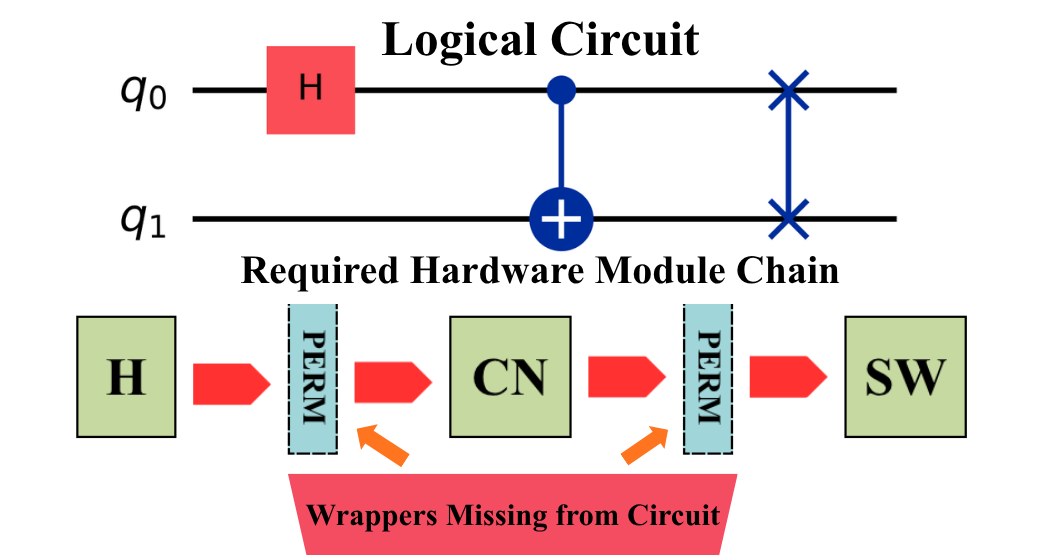
\includegraphics[width=0.6\columnwidth]{fig/fig2_composition.png}
    \caption{A 2-qubit circuit (top) and the module chain that the gate
    library requires for it (bottom). The CNOT module has its control on
    $q_1$, so \texttt{cx}$(q_0,q_1)$ is bracketed by permutation modules
    that do not appear in the circuit. The circuit was built in IBM Quantum
    Composer~\cite{composer} and drawn with Qiskit.}
    \label{fig:composition}
\end{figure}
   \setlength{\textfloatsep}{8pt plus 2pt minus 2pt}

As a result, three circuit families are constructed and evaluated using the same design methodology. As summarized in Table~\ref{tab:circuit_fam}, the first family consists of 2-qubit circuits obtained through wire cutting~\cite{liu2026wirecut,hpdc26}. The second family is based on the 3-qubit quantum Fourier transform (QFT)~\cite{isqed2026} and utilizes its gates: Hadamard, controlled-$S$, controlled-$T$, and SWAP. The third family focuses on 5-qubit GHZ-state preparation, comprising a Hadamard gate followed by a chain of CNOT gates~\cite{isqed2026}, and uses only Hadamard and CNOT gates. Each family also includes circuits developed for this work or authored in IBM Quantum Composer~\cite{composer}, which employ the same gates and gate library. %The circuits placed and routed on the FPGA are summarized in Table~\ref{tab:circuit_fam}.

% Required packages: \usepackage{booktabs,tabularx}
\begin{table}[ht]
\centering
\caption{Circuit families and complexity.}
\label{tab:circuit_fam}
\begin{tabular*}{\linewidth}{@{\extracolsep{\fill}}llccc@{}}
\toprule
Benchmarks & Circuits & Width & Depth & Gates \\
\midrule
Circuit Cut~\cite{hpdc26} & \texttt{Circuit0\_06}   & 2 & 2 & 2 \\
Circuit Cut~\cite{hpdc26} & \texttt{Circuit0\_17}   & 2 & 2 & 3 \\
Circuit Cut~\cite{hpdc26} & \texttt{Circuit0\_2}    & 2 & 2 & 3 \\
Circuit Cut~\cite{hpdc26} & \texttt{Circuit0\_3}    & 2 & 3 & 4 \\
Circuit Cut~\cite{hpdc26} & \texttt{Circuit0\_4}    & 2 & 2 & 3 \\
Circuit Cut~\cite{hpdc26} & \texttt{Circuit0\_5}    & 2 & 3 & 4 \\
Circuit Cut~\cite{hpdc26} & \texttt{Circuit1\_0167} & 2 & 2 & 2 \\
Circuit Cut~\cite{hpdc26} & \texttt{Circuit1\_23}   & 2 & 3 & 3 \\
Circuit Cut~\cite{hpdc26} & \texttt{Circuit1\_45}   & 2 & 3 & 3 \\
QFT3~\cite{isqed2026} & \texttt{QFT}                & 3 & 6 & 7 \\
GHZ~\cite{isqed2026} & \texttt{ShorFixed}$^\ddag$   & 5 & 5 & 5 \\
IBM Composer~\cite{composer} & \texttt{U3\_5}       & 3 & 3 & 4 \\
GHZ variant (this work) & \texttt{G5\_05}           & 5 & 3 & 3 \\
IBM Composer~\cite{composer} & \texttt{V5\_6}       & 5 & 1 & 3 \\
\bottomrule
\end{tabular*}

\vspace{2pt}
\parbox{\linewidth}{\footnotesize Width is the number of qubits; depth and
gate count are as reported by Qiskit. $^\ddag$The corrected GHZ reference
(Section~\ref{subsec:defects}), not a generated design.}
\end{table}

%================
\section{Prompt Generation}
This section evaluates the effectiveness of hardware generation across varying levels of prompt detail, from full to sparse, circuit complexities, and the inclusion or omission of library documentation in the prompts. It also analyzes the resulting failures.

\subsection{Prompt-Only Generation Study}
\label{subsec:prior}

The prompt-only study was conducted to characterize how an LLM fails when provided with only a prompt. The study was designed as a grid
over 11 circuits (the nine 2-qubit circuits, the QFT, and the 5-qubit GHZ circuit), two specification formats (Python and JSON), four levels of prompt detail, three models, and five repetitions per cell.

The four prompt levels differ in the hardware knowledge they provide. Every
prompt contains the circuit specification and a fixed task instruction that
gives the module interface and the output format. 

\begin{itemize}
    \item The \emph{full} level
adds four attachments, which are a gate-library listing, the architectural
rules, the pipeline sequence, and hints for the permutation modules. 
\item The
\emph{medium} and \emph{medium-strict} levels withdraw these attachments
progressively, and the medium-strict level additionally tightens the
wording of the instruction. 
\item The \emph{sparse} level withdraws all four
attachments, leaving only the circuit and the task. 
\end{itemize}

\subsection{Generation Analysis: Pass Rate V.S. Prompt levels}
In what follows, each design was compiled and simulated in \textit{ModelSim} simulator against golden amplitudes obtained by
simulating the corresponding reference design, and 372 of the 661 designs
passed. Because not every cell of the grid was completed, the three \textit{Gemini} models
contribute very different numbers of runs, and no conclusion about model
ranking is drawn.

As illustrated in Table~\ref{tab:phase1grid}, prompt detail had the largest effect on the pass rate. At the sparse level 29.2\% of designs passed, compared with 88.2\% at the full level. This difference holds within each model considered separately (0.0\% to 83.3\%, 0.0\% to 81.8\%, and 40.9\% to 91.9\%),
although the smallest of the sparse cells contains only four runs. The
specification format had little effect, with 189 of 330 Python runs and 182 of 330 \textit{JSON} runs passing.

\begin{table}[ht]
\centering
\caption{Prompt-only study: designs passing simulation, by model and prompt level, over all 661 runs. }
\label{tab:phase1grid}
\begin{tabular}{@{}lrrrr@{}}
\toprule
Model & Full & Medium & Medium-strict & Sparse \\
\midrule
3.1-flash-lite & 35/42 & 51/78 & 21/78 & 0/40 \\
3.5-flash & 68/74 & 54/74 & 85/110 & 45/110 \\
3.1-pro-preview & 9/11 & 0/20 & 4/20 & 0/4 \\
\midrule
All models & 112/127 & 105/172 & 110/208 & 45/154 \\
\bottomrule
\end{tabular}
\end{table}

%Cells are unevenly filled because not every cell of the grid was completed, and the three models therefore carry very different totals (238, 368 and 55 runs); the counts are given so each cell can be read with its own $n$. Within every model the effect of prompt detail is in the same direction. We draw no ranking between models from this table: the model with the best full-prompt cell on the hard circuits, 3.1-pro-preview, has the weakest overall record (13/55).

\subsection{Generation Analysis: Pass Rate V.S. Circuit Complexity}
Moreover, Figure~\ref{fig:phase1cliff} illustrates that the amount of prompt detail required depends on circuit size. The 2-qubit circuits pass at every level,
including 45 of the 126 runs that received no hardware knowledge. In
contrast, the 3- and 5-qubit circuits pass in only 4 of 120 runs below the
full level. Hardware knowledge that is optional for 2-qubit circuits is
therefore close to mandatory for the larger families, and the system
described in Section~\ref{sec:system} is designed to supply it.

\begin{figure}[ht]
    \centering
    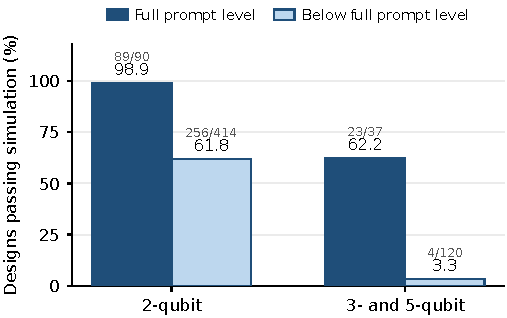
\includegraphics[width=0.8\columnwidth]{fig/phase1_cliff.pdf}
    \caption{Prompt-only study: pass rate at the full prompt level and at
    all lower levels combined, by circuit size. The four passing 3- and
    5-qubit runs below the full level all fall in one intermediate level.}
    \label{fig:phase1cliff}
\end{figure}

The 5-qubit verdicts of this study are subject to one limitation. The
5-qubit GHZ reference is defective 
(Section~\ref{subsec:defects}), and the study simulated it using the
all-zero input, which the defect leaves unchanged. Therefore, the study could not have detected that defect.

\subsection{Prompt Analysis of library utilization}
Table~\ref{tab:conformance} shows that library use alone does not guarantee correctness. Among the 460 designs with retained source code, every design generated with library documentation instantiated library modules, while none generated without it did so. In these experiments, library adoption followed the availability of documentation in the prompt. However, 111 of the 341 designs using library modules failed simulation, while 45 of the 117 designs implementing gate arithmetic inline passed. Library use was thus neither sufficient nor necessary for simulation correctness, although it was associated with a higher pass rate: 67.4\% (230/341), compared with 38.5\% (45/117) for inline implementations.

\begin{table}[ht]
\centering
\caption{Prompt-only study: library use and simulation outcome for the 460 retained designs. Two designs in neither class are omitted.}
\label{tab:conformance}
\begin{tabular}{@{}lrrr@{}}
\toprule
Prompt level & Library-conformant & From scratch & Passed \\
\midrule
Full & 78 & 0 & 66/78 \\
Medium & 112 & 0 & 68/112 \\
Medium-strict & 151 & 0 & 96/151 \\
Sparse & 0 & 117 & 45/117 \\
\midrule
All & 341 & 117 & 275/458 \\
\bottomrule
\end{tabular}
\end{table}


\subsection{Failures Analysis}
As shown in Table~\ref{tab:failures}, failures are classified automatically when the simulation logs clearly identify the cause and manually otherwise. A single design could receive multiple failure tags. Incorrect output amplitudes were the most common failure class, followed by omitted permutation wrappers and references to nonexistent modules. The latter two classes together accounted for 145 tagged runs and are the focus of the proposed system (Section~\ref{sec:system}).
\begin{table}[ht]
\centering
\caption{Prompt-only study: failure classes over the 289 failing runs. A run can carry several tags; four tags occurring once each are omitted. The full tally is the \texttt{error\_types} column of the study's run record, \texttt{runs\_matched\_arms.csv}.}
\label{tab:failures}
\begin{tabular}{@{}lr@{}}
\toprule
Failure class & Runs tagged \\
\midrule
Wrong output amplitudes & 169 \\
Omitted permutation wrapper & 78 \\
Module that does not exist & 67 \\
Wrong gate decomposition & 27 \\
Syntax error & 25 \\
Mismatched port name & 11 \\
Unstable valid protocol & 7 \\
Implicit net declaration & 4 \\
Multiply driven wire & 3 \\
\bottomrule
\end{tabular}
\end{table}

%One run can carry several tags, so the column sums past 289. Tagging was automatic where the log made the cause unambiguous and by hand otherwise. The second and third rows are the classes the system of Section~\ref{sec:system} targets: neither can be reasoned out from the circuit.

% =====================================================================
% IV. PROPOSED SYSTEM
% =====================================================================
\section{Proposed System and Framework}
\label{sec:system}
This section presents the workflow for the hardware generation and evaluation. 

\subsection{Overall Workflow}
Figure~\ref{fig:llm-verilog-workflow} illustrates the overall workflow. An LLM translates a \textit{Qiskit} circuit into a hardware design composed of gate library modules. The design is then simulated to verify its functionality. Designs that pass verification proceed to FPGA synthesis and implementation.

Generation comprises five stages: legality screening, prompt assembly using two types of context, an initial call to \texttt{gemini-3.5-flash} at temperature~0, static linting, and up to two lint-driven repair calls. Functional verification is performed separately, and its results are not fed back to the generator. The framework also supports a local open-model backend, \textit{Qwen2.5-Coder-7B}, served through \textit{Ollama}. All results reported in this paper are obtained using \texttt{gemini-3.5-flash}. In the only recorded trial using the \textit{Qwen} backend, the generated designs omitted the required permutation wrappers, and the repair step failed to restore them.

\begin{figure*}[t]
    \centering
    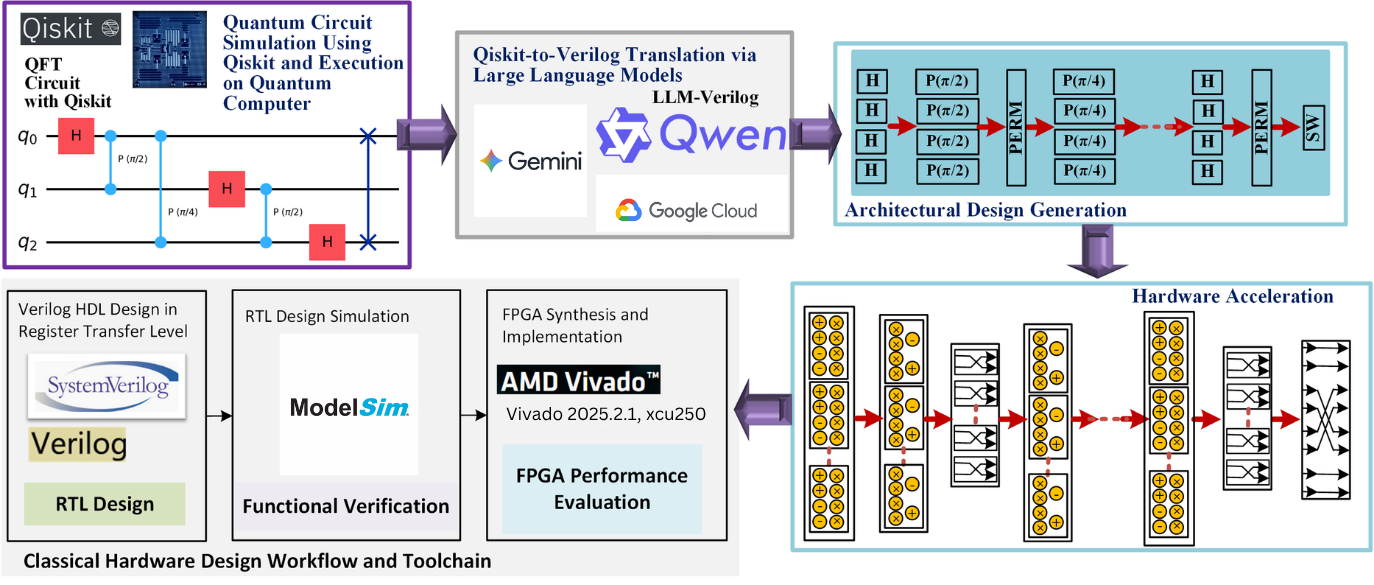
\includegraphics[width=.9\linewidth]{fig/llm-verilog-workflow.png}
    \caption{Workflow of the proposed approach: an LLM translates a Qiskit
    circuit into a top-level design over the gate library, which is
    verified in ModelSim and synthesized in Vivado. All results reported in
    this paper use \texttt{gemini-3.5-flash}, and the Qwen2.5-Coder-7B
    backend shown is not evaluated.}
    \label{fig:llm-verilog-workflow}
\end{figure*}

\begin{comment}
\subsection{Problem Setup and Output Target}
\label{subsec:setup}
Specifically, the input is a \textit{Qiskit} circuit, provided either as a Python script or as a
\texttt{.qpy} container, which is converted to a canonical gate list. The
output is a single module that instantiates library modules and chains
their ports, and that contains no gate logic of its own. Each family has a fixed set of legal gates,
determined by the modules that the library provides. The 2-qubit family
supports \texttt{h}, \texttt{x}, \texttt{sx}, \texttt{sxdg}, \texttt{swap},
and \texttt{cx}. The 3-qubit QFT family supports \texttt{h}, \texttt{cs},
\texttt{cp($\pi/4$)} (a controlled-$T$ gate), and \texttt{swap}. The
5-qubit family supports only \texttt{h} and \texttt{cx}. A circuit that
uses any other gate is rejected, and no approximation is attempted.


\subsection{Non-Derivable Library Knowledge}
\label{subsec:nonderivable}
Specifically, the input is a \textit{Qiskit} circuit, provided either as a Python script or as a
\texttt{.qpy} container, which is converted to a canonical gate list. The
output is a single module that instantiates library modules and chains
their ports, and that contains no gate logic of its own. Each family has a fixed set of legal gates,
determined by the modules that the library provides. Four facts about this library cannot be inferred from a circuit, and the
first three account for failure classes observed in the prompt-only study, as illustrated in section~\ref{subsec:prior}. 
\end{comment}

\begin{comment}
First, the permutation modules are numbered
with gaps. Variants \texttt{\_7} and \texttt{\_8} do not exist, and the
5-qubit family provides only nine of the ten possible qubit exchanges. The
missing exchange, between qubits 2 and 3, must therefore be routed through
qubit 4 as \texttt{\_9}, \texttt{\_10}, \texttt{\_9}, and a model that
guesses \texttt{\_7} instantiates a module that does not exist. Second, the
2-qubit CNOT module is wired with the control on $q_1$ and the target on
$q_0$. As a result, \texttt{cx(0,1)} requires a permutation bracket
(Fig.~\ref{fig:composition}), whereas \texttt{cx(1,0)} must not have one.
Bracketing the wrong case produces a different gate from the correct
modules, which would appear as incorrect output amplitudes. Third, the
controlled-$S$ module lacks two of the input ports that the other gate
modules have, because they were removed by the synthesis toolchain, so a
port list inferred by analogy is incorrect. Fourth, the fixed-point format
differs between families. These facts are therefore supplied to the model
directly.
\end{comment}
\begin{comment}
\subsection{Non-Derivable Library Knowledge}
\label{subsec:nonderivable}
The input to the system is a \textit{Qiskit} circuit, given as a Python
script or a \texttt{.qpy} file, and the output is a single top-level module
that instantiates library modules and connects their ports without adding
gate logic of its own. Each family accepts only the gates for which the
library has modules: \texttt{h}, \texttt{x}, \texttt{sx}, \texttt{sxdg},
\texttt{swap}, and \texttt{cx} for the 2-qubit family; \texttt{h},
\texttt{cs}, \texttt{cp($\pi/4$)}, and \texttt{swap} for the 3-qubit
family; and \texttt{h} and \texttt{cx} for the 5-qubit family.

Three facts about the library cannot be inferred from a circuit, and each
matches a failure class in Table~\ref{tab:failures}. First, the permutation
modules of Fig.~\ref{fig:composition}, named
\texttt{CompatiblePerm\_}$k$, each exchange one pair of qubits and are
numbered with gaps: variants \texttt{\_7} and \texttt{\_8} do not exist,
and the 5-qubit family has modules for only nine of its ten qubit pairs.
The missing exchange, of qubits 2 and 3, must be built from three
available ones, \texttt{CompatiblePerm\_9}, \texttt{\_10}, \texttt{\_9},
which route it through qubit~4. Second, the 2-qubit CNOT module has its
control on $q_1$, so \texttt{cx(0,1)} needs a permutation before and after
it (Fig.~\ref{fig:composition}), whereas \texttt{cx(1,0)} must not have
one. Third, the controlled-$S$ module lacks two input ports that the other
modules have, so a port list copied by analogy is wrong. These facts are
therefore given to the model in every prompt.
\end{comment}
\subsection{Prompt Context Construction}
\label{subsec:paths}

Knowledge reaches the model through two paths. The first is the
always-injected context, which is included in full in every prompt and has
three parts. These are a gate reference covering all families, the module
interfaces of the target family, which are extracted from the reference
register-transfer level (RTL) code so that every port name is exact, and
the composition rules of the family, which were derived by hand from
measurements of the behavior of each module. 

The second path is the
retrieved context, which consists of exactly one worked example selected
from the corpus by structural similarity. The similarity score is a
weighted sum of sequence ratios over the pattern of permutation brackets
(0.60), the qubit-target sequence (0.30), and the gate-name sequence
(0.10). Retrieval is leave-one-out, so a corpus circuit never retrieves
itself. The retrieved example is condensed to its module sequence and one
verbatim instantiation block, which serves as a formatting sample, and its
full port connections are omitted. The prompt is assembled in a fixed
order, consisting of the gate reference, the interfaces, the composition rules, the
example, the circuit to be implemented, and the task. The resulting prompt
contains 3,688--4,026 input tokens for a 2-qubit circuit, 2,979--4,266 for
a 3-qubit circuit, and 9,076--9,314 for a 5-qubit circuit.

\subsection{Legality Screening, Lint, and Repair}
\label{subsec:screening}

Two screens are applied before any model call. The first is a gate-set
check, which rejects circuits that use gates outside the legal set of the
family. The second is the \emph{H-safety} screen, which addresses a library
defect reported in Section~\ref{subsec:correctness}, namely that the
Hadamard module of the 2-qubit family misreads negative amplitudes. A basis
input is \emph{H-safe} for a circuit if, when the ideal amplitudes of the
circuit are followed from that input, no Hadamard gate receives a negative
component. A circuit is scored only from an input that is both H-safe and \emph{discriminating}, meaning that its golden state distinguishes the two basis states that a qubit exchange would swap. A circuit for which no such input exists is excluded, because scoring it would measure the defect in the library and not the quality of the generation. 

% %A circuit is scored only from an input that is both H-safe and \emph{discriminating}, meaning that its golden state distinguishes the two basis states that a qubit exchange would swap. A circuit for which no such input exists is excluded, because scoring it would measure the defect in the library and not the quality of the generation. The screen applies this rule to every family, although the sign defect is confined to the 2-qubit library. The 3- and 5-qubit modules sign-extend correctly, so exclusions in those families are conservative with respect to that defect. They are not without effect, however, because the 8-bit Hadamard module still rounds negative amplitudes downward, and Section~\ref{subsec:ablation} reports a case in which that rounding alone exceeds the $\pm1$~LSB tolerance. Section~\ref{subsec:limitations} discusses the one circuit affected.

After generation, a static lint applies six checks to the emitted module.
The checks verify that (i) every instantiated module exists and can be
instantiated at the top level, (ii) the top-level port list is complete,
(iii) each instance connects only ports that exist and leaves no required
port unconnected, (iv) the stages chain from the top-level inputs to the
outputs, (v) no wire is declared twice, and (vi) the number of
instantiations matches the number derived from the composition rules. Any finding is
returned to the model as a repair prompt, at most twice, so that a circuit
requires at most three model calls. The lint serves only as a filter that
runs before simulation, and it does not determine correctness.

% =====================================================================
% V. EVALUATION METHODOLOGY
% =====================================================================

\begin{comment}
    
\section{Evaluation Methodology}
\label{sec:method}

\subsection{Limitations of Structural Comparison}
\label{subsec:structural}
%None of the benchmarks cited in this paper scores designs in this way, since VerilogEval and RTLLM both simulate against a testbench written for each task~\cite{verilogeval2023,rtllm2024}. 
A structural check compares the generated top-level design against a
reference and requires that the same modules are instantiated in the same
order. Such a check is inexpensive and requires no simulator. A structural check is nevertheless the only option available when a reference exists and a functional verdict
does not, and this paper reports one such structural match for the single
circuit that the input screen leaves unscored
(Section~\ref{subsec:limitations}). A structural check has two blind spots.
It cannot determine whether the reference itself is correct, and it cannot
determine whether a design that is wired differently from the reference
computes the correct state.

The second blind spot is demonstrated by the prompt-only study, in which 45
designs that instantiated no library module at all nevertheless passed
simulation (Section~\ref{subsec:prior}). The 111 conformant designs that
failed are not evidence of the same point, because the classification used
there records only whether library modules were used and not whether they
appear in the order of the reference. The first is demonstrated by the 5-qubit
reference implementation of this project, which ends with one permutation
too many and consequently leaves two qubits exchanged. The input from which
this reference was customarily tested is unchanged by that exchange, so the
defect was never observed. A structural comparison against this reference
would certify as correct every generated design that reproduced the defect.
The corresponding measurements are given in Section~\ref{subsec:defects}.
\end{comment}



% =====================================================================
% VI. EXPERIMENTAL RESULTS
% =====================================================================
\section{Experimental Results}
\label{sec:results}
This section introduces the simulation and performance evaluation results. All circuits are generated by \texttt{gemini-3.5-flash} at temperature~0
and simulated in \textit{ModelSim}. The 14 designs of Table~\ref{tab:circuit_fam} are implemented using Vivado 2025.2.1 for the
\texttt{xcu250-figd2104-2L-e} device of the AMD Alveo U250 card~\cite{yang2024integrated}.
\begin{comment}
\subsection{Statevector Verification}
\label{subsec:statevector}
Each generated design is checked against a golden state computed from the
circuit specification. \textit{Qiskit} evolves a basis input exactly
through the circuit, \textit{ModelSim} simulates the generated design from
the same input, and the two outputs are compared component by component.
No reference hardware design is involved. A component passes if it lies
within $\pm16$~LSB in Q2.14 or $\pm1$~LSB in Q1.7. The 16-LSB bound was set
empirically to absorb the truncation error of the library and is not
derived analytically. Outputs are read 128 clock cycles after the
output-valid flag is raised, because the reference QFT raises that flag
before its data has settled (Section~\ref{subsec:defects}).

The screened input of Section~\ref{subsec:screening} can reveal an error in
only one of the $\binom{n}{2}$ possible qubit exchanges of an $n$-qubit
design. Every 3- and 5-qubit design is therefore also simulated from a
\emph{covering set} of H-safe inputs that together detect an error in any
qubit exchange. For \texttt{V5\_6}, no H-safe input detects the exchange of
qubits 2 and 3, and that exchange is examined separately in
Section~\ref{subsec:route}. The 2-qubit designs have only one qubit pair
and need no covering set.
\end{comment}

\subsection{Experimental Setup and Functional Verification}
\label{subsec:correctness}
Table~\ref{tab:results} presents functional correctness by evaluation set.
The held-out and supplied circuits were authored in IBM Quantum
Composer~\cite{composer}, and their golden states were computed by the
harness. Of the 55 evaluated circuits, 53 produce hardware whose simulated
output amplitudes match the \textit{Qiskit} golden state within a fixed-point
tolerance of $\pm16$~LSB per component in Q2.14 and $\pm1$~LSB in Q1.7,
resulting in a pass rate of 96.4\%. On average, generation required
1.07 attempts per circuit. Only two circuits required more than
one attempt, namely \texttt{G5\_05} and the supplied circuit
\texttt{V5\_0}, and both belong to the 5-qubit family.

\begin{table}[ht]
\centering
\caption{Functional results by evaluation set. }
\label{tab:results}
\begin{tabular}{@{}llrr@{}}
\toprule
Evaluation set & Family & Circuits & Passed \\
\midrule
Corpus (leave-one-out) & 2-qubit & 9 & 9 \\
Held-out (NC, independent) & 2-qubit & 9 & 9 \\
Novel (GEN, profile-covering) & 2-qubit & 12 & 11 \\
Novel (G3, qft family) & 3-qubit & 8 & 7 \\
Novel (G5, GHZ family) & 5-qubit & 5 & 5 \\
Supplied (.qpy, user-authored) & 3-qubit + 5-qubit & 12 & 12 \\
\midrule
Total & & 55 & 53 \\
\bottomrule
\end{tabular}
\end{table}


The first failure, \texttt{GEN\_02}, is caused by an existing arithmetic
defect in the gate library and not by the generation: the Hadamard module of
the 2-qubit family misreads negative amplitudes, resulting in the circuit producing one
in hardware, even though its ideal state contains none. The second failure, \texttt{G3\_06}, is a generation error that was not visible from the screened input. The specification is \texttt{swap(0,1)} followed by \texttt{h(0)}. The model emitted the swap module, then
\texttt{CompatiblePerm\_2}, which exchanges qubits 0 and 1 a second time,
and then the Hadamard module, so that the swap is cancelled. Because a swap
leaves $|000\rangle$ unchanged, the design passed from its screened input.
Every 3- and 5-qubit design was also re-simulated from a \emph{covering
set}, a set of H-safe inputs that together detect an error in any qubit
exchange (for \texttt{V5\_6}, every exchange except that of qubits 2 and 3).
The covering set exposed the error in \texttt{G3\_06} with deviations of up
to 91~LSB, and the remaining 24 designs of the 3- and 5-qubit families
matched their covering sets within 1~LSB.

Three circuits are not included in the 55: the held-out circuit
\texttt{NC\_02}, for which no input is both H-safe and discriminating
(Section~\ref{subsec:screening}); \texttt{G5\_03}, which exceeds the model's output
limit; and the full 3-qubit QFT, which remains unscored by the same screen.

%In the 2-qubit family, the \texttt{SplitMultiplier} module zero-extends a signed value, so that a negative amplitude is read as a large positive one. The 3- and 5-qubit modules sign-extend the same value and are unaffected. In this hardware, \texttt{sx} followed by \texttt{sxdg} composes to $-I$, and the resulting negative amplitude corrupts the output of the Hadamard gate that follows. The H-safety screen cannot detect this case, because the ideal state contains no negative component. This attribution rests on the arithmetic mechanism just described. The generated composition also matches the composition rules exactly, although Section~\ref{subsec:structural} notes that such a match cannot by itself establish correctness.

%This is the same defect that prompted the first revision of the composition rules (Section~\ref{subsec:limitations}). Because a swap leaves $|000\rangle$ unchanged, the design passed all 16 component checks from that input. From the covering set, the design fails at $|001\rangle$, where four components deviate by up to 91~LSB and the output is within 1~LSB of that of the Hadamard gate applied alone. The remaining 24 designs of the 3- and 5-qubit families match their golden states from their covering sets, with no component deviating by more than 1~LSB (Table~\ref{tab:coverage}). For \texttt{V5\_6}, the one exchange that no H-safe input can detect is tested separately in Section~\ref{subsec:ablation}.

%Three circuits are not included in the 55. For \texttt{NC\_02}, no input is both H-safe and discriminating (Section~\ref{subsec:screening}), so no simulation could distinguish a correct implementation from an incorrect one. \texttt{G5\_03} could not be generated, because it exceeds the output limit of the model (Section~\ref{subsec:limitations}). The full 3-qubit QFT was generated but is left unscored by the same screen that excludes \texttt{NC\_02}, and is discussed in Section~\ref{subsec:limitations}.

\subsection{Hardware Cost and Performance Evaluation}
\label{subsec:hardware}

%\begin{table}[ht]
\centering
\caption{Covering-set re-simulation of every 3- and 5-qubit design. Each design is re-run from a set of H-safe basis inputs whose golden states jointly distinguish all $\binom{n}{2}$ qubit exchanges. \texttt{G3\_06} is the one design this catches: it passed 16/16 from its screened input and misses by 91~LSB from the covering set. Every other design is within 1~LSB on every component. \texttt{V5\_6} is the one design whose set is incomplete---no H-safe input distinguishes the 2--3 exchange---and it is treated separately in Table~\ref{tab:route}.}
\label{tab:coverage}
\begin{tabular}{@{}llrrr@{}}
\toprule
Set & Family & Designs & Exchanges & Max err. (LSB) \\
\midrule
G3 & 3-qubit, generated & 8 & 3/3 & 91 \\
U3 & 3-qubit, supplied & 6 & 3/3 & 1 \\
G5 & 5-qubit, generated & 5 & 10/10 & 1 \\
V5 & 5-qubit, supplied & 6 & 10/10 (1 at 9/10) & 1 \\
\bottomrule
\end{tabular}
\end{table}

Hardware resource utilization is evaluated on the AMD Alveo U250 data center accelerator card for all 14 circuits of Table~\ref{tab:circuit_fam}. As shown in Table~\ref{tab:hardware}, look-up tables (LUTs) and digital signal processing (DSP) blocks primarily perform arithmetic logic, and flip-flops (FFs) provide pipeline registers. The 2-qubit designs utilize 128 to 450 LUTs, while the 3- and 5-qubit designs use 878 to 5,775 LUTs. Dynamic power (DP) consumption is on the order of hundreds of milliwatts, and the maximum operating frequency (MOF) ranges from 416 to 828~MHz. The three 5-qubit designs (marked $^\dag$) are synthesized out-of-context because their 1,028 pins exceed the 676 pins available from the device, and their lower dynamic power, despite containing more logic, is consistent with having no I/O placed. Out-of-context timing is internally accurate and comparable across these three designs, but is not guaranteed once a design is encapsulated by surrounding circuitry; therefore, their reported frequencies should be read as upper bounds.

%Fourteen designs were placed and routed on the target device. Thirteen of them were generated, comprising the nine 2-qubit corpus circuits, the full QFT, \texttt{U3\_5}, \texttt{G5\_05}, and \texttt{V5\_6}. The fourteenth is \texttt{ShorFixed}, the corrected 5-qubit reference described in Section~\ref{subsec:defects}, which retains its original file name. The nine 2-qubit designs use between 128 and 450 LUTs and between 261 and 954 flip-flops. Table~\ref{tab:hardware} reports the 3- and 5-qubit designs. The 5-qubit designs were synthesized out-of-context, because a 5-qubit top-level design presents 1,028 pins, whereas the device provides 676. Three of the fourteen designs, \texttt{U3\_5}, \texttt{G5\_05}, and \texttt{V5\_6}, have no reference implementation, and no prior design is available for comparison.

\begin{table}[ht]
\centering
\footnotesize
\setlength{\tabcolsep}{4pt}
\caption{Hardware cost of all 14 placed and routed designs.}
\label{tab:hardware}
\begin{tabular}{@{}lcrrrrr@{}}
\toprule
Circuit & $n$ & LUTs & FFs & DSPs & DP (W) & MOF (MHz) \\
\midrule
Circuit0\_06 & 2 & 128 & 261 & 16 & 0.607 & 659 \\
Circuit0\_17 & 2 & 129 & 648 & 16 & 0.604 & 784 \\
Circuit0\_2 & 2 & 257 & 651 & 32 & 0.647 & 674 \\
Circuit0\_3 & 2 & 257 & 652 & 32 & 0.639 & 661 \\
Circuit0\_4 & 2 & 449 & 825 & 16 & 0.618 & 690 \\
Circuit0\_5 & 2 & 449 & 954 & 16 & 0.624 & 605 \\
Circuit1\_0167 & 2 & 130 & 517 & 16 & 0.602 & 828 \\
Circuit1\_23 & 2 & 258 & 520 & 32 & 0.640 & 613 \\
Circuit1\_45 & 2 & 450 & 838 & 16 & 0.622 & 651 \\
QFT & 3 & 1,273 & 1,940 & 52 & 0.716 & 469 \\
ShorFixed$^\dag$ & 5 & 2,272 & 7,183 & 64 & 0.299 & 578 \\
U3\_5 & 3 & 878 & 1,229 & 36 & 0.660 & 479 \\
G5\_05$^\dag$ & 5 & 1,760 & 4,105 & 64 & 0.184 & 536 \\
V5\_6$^\dag$ & 5 & 5,775 & 5,133 & 192 & 0.583 & 416 \\
\bottomrule
\end{tabular}
\end{table}


%Static power lies between 2.948 and 2.958\,W for every design and is determined by the device. The maximum operating frequency varies with placement and routing. Neither quantity is therefore a stable basis for comparing designs.

Table~\ref{tab:cycles} reports the latency in clock cycles, measured from
the first clock edge when the input-valid flag is high to the first clock
edge when the output-valid flag is high. All ten generated designs that match the reference have latency
 that coincides exactly, and they instantiate the same modules
in the same order as the reference. \texttt{ShorFixed} is not a generated
design but the corrected 5-qubit reference (Section~\ref{subsec:defects}),
 taking 17 cycles compared to 18 for the original.
\texttt{U3\_5}, \texttt{G5\_05}, and \texttt{V5\_6} have no reference for
 comparison.

\begin{table}[ht]
\centering
\caption{Latency in clock cycles.}
\label{tab:cycles}
\begin{tabular}{@{}lrrr@{}}
\toprule
Circuit & Chisel (cycles) & Generated (cycles) & Difference \\
\midrule
Circuit0\_06 & 5 & 5 & 0 \\
Circuit0\_17 & 8 & 8 & 0 \\
Circuit0\_2 & 11 & 11 & 0 \\
Circuit0\_3 & 12 & 12 & 0 \\
Circuit0\_4 & 9 & 9 & 0 \\
Circuit0\_5 & 10 & 10 & 0 \\
Circuit1\_0167 & 7 & 7 & 0 \\
Circuit1\_23 & 11 & 11 & 0 \\
Circuit1\_45 & 9 & 9 & 0 \\
QFT & 20 & 20 & 0 \\
Shor / ShorFixed & 18 & 17 & $-1$ \\
U3\_5 & -- & 13 & -- \\
G5\_05 & -- & 9 & -- \\
V5\_6 & -- & 15 & -- \\
\bottomrule
\end{tabular}
\end{table}


\subsection{Defect in the 5-Qubit Reference}
\label{subsec:defects}
The 5-qubit GHZ reference ends with a redundant \texttt{CompatiblePerm\_10},
 leaving qubits 3 and 4 exchanged and adding one pipeline stage. The
defect went unnoticed because the inputs from which the reference had been tested
, $|00010\rangle$ and the all-zero input of the prompt-only study, are
unchanged by that exchange. From $|10000\rangle$, the reference fails 4 of
its 64 amplitude components, while the corrected design,
\texttt{ShorFixed}, passes all 64 from both inputs. A structural
comparison, which judges a generated design as correct if it instantiates the
same modules as a reference in the same order, would have accepted every
generated design that copied this defect.

\begin{comment}
\subsection{Defects Exposed by Simulation}
\label{subsec:defects}
The evaluation exposed three defects in artifacts that had previously been
assumed correct. The sign-extension defect in the 2-qubit multiplier is
described in Section~\ref{subsec:correctness}, and the timing defect in the
handshake of the reference QFT is described in
Section~\ref{subsec:statevector}. This subsection reports the third defect,
together with a false positive in the static lint of the proposed system.

The 5-qubit reference implementation contains a defect in its closing
permutation cascade. The final \texttt{CompatiblePerm\_10} instantiation is
redundant and leaves qubits 3 and 4 exchanged. The defect had not been
observed because the input from which the evaluation harness simulates this
circuit by default, $|00010\rangle$, is invariant under that exchange, as is
the all-zero input used in the prompt-only study
(Section~\ref{subsec:prior}). From $|00010\rangle$, the reference with 16
instantiations passes all 64 component checks.
From $|10000\rangle$, which was selected to be sensitive to the exchange,
the reference fails 4 of the 64 checks. The corrected design with 15
instantiations passes all 64 checks from both inputs. Of the 32 basis
inputs, 16 are both H-safe and sensitive to the exchange, and none of them
had previously been used. The defect also added a pipeline stage, since the
corrected design is one cycle faster (Section~\ref{subsec:hardware}).

The static lint produced one false positive. Its chain check compared
signals by position, so that valid 3-qubit designs using the controlled-$S$
module, which lacks two input ports, were rejected. The three affected
circuits exhausted their repair budget on this finding and subsequently
passed simulation, which indicated that the fault lay in the check. The
verdicts were unaffected, and correcting the check reduced the average
number of attempts per circuit from 1.18 to 1.07.


\subsection{Context Ablation}
\label{subsec:ablation}

\begin{table}[ht]
\centering
\caption{Context ablation on the 9 held-out 2-qubit circuits, one section withheld per run at the same model and temperature. Only row 5 changes the outcome: interface knowledge is supplied twice, in the interfaces document and in the worked example, so withholding either alone leaves the other. Every condition reaches 9/9 after repair.}
\label{tab:ablation}
\begin{tabular}{@{}clrrr@{}}
\toprule
\# & Context withheld & pass@1 & Lint err. & Final \\
\midrule
1 & None (full context) & 9/9 & 0 & 9/9 \\
2 & Module interfaces & 9/9 & 0 & 9/9 \\
3 & Composition rulebook & 9/9 & 0 & 9/9 \\
4 & Worked example & 9/9 & 0 & 9/9 \\
5 & \textbf{Example \emph{and} interfaces} & \textbf{0/9} & \textbf{5--17} & \textbf{9/9} \\
\bottomrule
\end{tabular}
\end{table}

\begin{table}[ht]
\centering
\caption{Generated \texttt{V5\_6} Against a Copy with the Route Removed.}
\label{tab:route}
\begin{tabular}{@{}llrrr@{}}
\toprule
Design & Input & Within tol. & Max err. (LSB) & Verdict \\
\midrule
Generated & $|00000\rangle$ & 64/64 & 0 & PASS \\
Generated & $|00100\rangle$ & 60/64 & 2 & FAIL \\
Generated & $|01000\rangle$ & 64/64 & 1 & PASS \\
Route removed & $|00000\rangle$ & 64/64 & 0 & PASS \\
Route removed & $|00100\rangle$ & 58/64 & 92 & FAIL \\
Route removed & $|01000\rangle$ & 60/64 & 91 & FAIL \\
\bottomrule
\end{tabular}
\end{table}


One section of the context was withheld per run for the nine held-out
2-qubit circuits, using the same model and temperature. Withholding the
interfaces document, the composition rules, or the worked example
individually left the first-attempt pass rate at 9/9 with no lint findings.
Interface knowledge is supplied twice, in the interfaces document and in
the verbatim instantiation block of the worked example, so removing either
source leaves the other available. Withholding the example and the
interfaces together reduced the first-attempt pass rate to 0/9, with 5--17
lint findings per circuit, and one round of repair recovered all nine
circuits. For the 2-qubit family, withholding any single section therefore
had no observable effect, and the context influenced the number of attempts
required and not the final outcome. The ablation was not repeated for the
3- and 5-qubit families.

One 5-qubit circuit suggests that the composition rules contribute more for
larger circuits. The supplied circuit \texttt{V5\_6} requires the one qubit
exchange for which the hardware has no module, which must be routed as
\texttt{CompatiblePerm\_9}, \texttt{\_10}, \texttt{\_9}
(Section~\ref{subsec:nonderivable}). Given the composition rules, the model
emitted exactly that route in nine instantiations and instantiated no
nonexistent module. The retrieved GHZ example contains \texttt{\_9} and
\texttt{\_10} but does not contain the sequence \texttt{\_9},
\texttt{\_10}, \texttt{\_9}, which originates from the composition rules.
The 5-qubit example held in the corpus is the original 16-instantiation
reference, that is, the version containing the defect reported in
Section~\ref{subsec:defects}. The route emitted for \texttt{V5\_6} therefore
did not come from the example.

Because \texttt{V5\_6} was scored from $|00000\rangle$, whose golden state
is unchanged by an exchange of qubits 2 and 3, a copy of the design with
the three route permutations removed was also simulated
(Table~\ref{tab:route}). From $|00000\rangle$, both designs match the
golden state exactly. From $|00100\rangle$ and $|01000\rangle$, which are
sensitive to the exchange, the generated design deviates by at most 2~LSB,
which is consistent with the 8-bit Hadamard module rounding negative
amplitudes down, whereas the copy without the route deviates by 91--92~LSB.
At $|00100\rangle$ the generated design exceeds the $\pm1$~LSB tolerance
and its verdict is therefore a failure. Neither $|00100\rangle$ nor
$|01000\rangle$ is H-safe for this circuit, so neither lies within the
scoring rule of Section~\ref{subsec:statevector} and neither contributes to
the result reported in Table~\ref{tab:results}. The route is consequently
supported by the difference in error magnitude between the two designs and
not by the verdict.

When the composition rules were withheld from this circuit, the generated
design did not compile. The model avoided the exchange by adopting a
different strategy, and the design failed on a duplicate wire declaration
and not on a nonexistent module. Of the three control circuits, one
required an additional round of repair. Since this observation rests on a
single circuit and the failure mechanism is a naming collision, it suggests
that the composition rules matter for larger circuits but does not
establish the reason.


% =====================================================================
% VII. LIMITATIONS
% =====================================================================
\section{Limitations}
\label{subsec:limitations}

\textbf{Revisions to the composition rules.} The composition rules were
revised twice during the evaluation. The first revision followed a 3-qubit
failure, \texttt{T\_01}, in which the model appended a permutation that
cancelled a logical swap. The rules of all three families were reworded to
distinguish a swap gate from a layout permutation. Four of the eight
3-qubit circuits were generated under the revised wording and are therefore
partly in-sample. The other four predate the revision, and one of them,
\texttt{G3\_06}, repeats the defect. The 5-qubit circuits were all
generated under the revised wording and passed 5/5. The second revision
added the route around the missing exchange after \texttt{G5\_03} could not
be generated. This route was first exercised by \texttt{V5\_6}, which was
supplied afterwards, and it has no out-of-sample check. The rules are
derived by hand from hardware measurements and are therefore specific to
this library.

\textbf{Model and repeatability.} All results were obtained with one model
at temperature~0 and one generation per circuit. The outputs were not
byte-identical across repeated runs. Of four circuits regenerated from an
identical prompt, one differed in text but not in module sequence. The
variance across repeated runs was not measured, and no claim across models
is supported.

\textbf{Output length.} For 5-qubit circuits, the output length of the
model is the limiting factor. Each instantiation carries 132 port
connections, and the circuit that could not be generated requires an
estimated 14--16 instantiations, whereas the largest design generated
successfully contains nine.

\textbf{Input coverage.} The 30 verdicts for 2-qubit circuits rest on a
single screened input (Section~\ref{subsec:statevector}), and
\texttt{G3\_06} shows that such an input can pass an incorrect design.

\textbf{Handshake timing.} Outputs are sampled 128 clock cycles after
\texttt{io\_out\_valid} is asserted (Section~\ref{subsec:statevector}). A
verdict therefore certifies the settled output values and not the timing of
the handshake. A generated design that asserted the flag early, as the
reference QFT does, would still be recorded as correct.

\textbf{The full QFT.} The full 3-qubit QFT has no functional verdict,
because no input is both H-safe and discriminating for it. The sign defect
against which the screen guards is confined to the 2-qubit library, and the
8-bit Hadamard module sign-extends (Section~\ref{subsec:screening}). A screen
restricted to the family that the defect affects would therefore admit inputs
for the QFT. Those inputs would, however, pass negative amplitudes through the
8-bit Hadamard, whose rounding can exceed the $\pm1$~LSB tolerance on its own
(Section~\ref{subsec:ablation}), so a failure from them could not be
attributed to the generation. Whether the QFT can be evaluated fairly
therefore remains open. The eight
3-qubit circuits in Table~\ref{tab:results} are simpler members of the same
family. The model did generate the full QFT without a worked example, and
the result matches the module sequence of the reference. This is a
structural match and does not constitute a functional verdict
(Section~\ref{subsec:structural}).
\end{comment}

%=======================
\section{Conclusion}
This paper evaluates LLM-assisted hardware generation for quantum circuit simulation and presents a hierarchical framework that combines explicit library knowledge, retrieved examples, and automated repair. The framework produces hardware implementations that align with reference simulation results for 53 of 55 circuits. FPGA evaluation further demonstrates the feasibility of the implementation and characterizes their performance and resource utilization. These findings support the viability of LLM-assisted, library-based hardware generation and emphasize the importance of explicit design knowledge, functional verification, and performance evaluation.

\section*{Acknowledgment}
We extend our gratitude to the National Science Foundation (NSF) for supporting this project under Award No. \#2512983 and \#2243981. 


\begin{thebibliography}{00}
\bibitem{ali2026fpga}
N. N. Ali, A. Tiwari, N. Khan, et al.,
``FPGA Based Quantum Circuit Simulator: Processing 30 Qubit Systems,''
\textit{Research Square}, preprint, version 1, Jan. 2026.

\bibitem{cicero2025simulation}
A. Cicero, M. A. Maleki, M. W. Azhar, A. F. Kockum, and P. Trancoso,
``Simulation of Quantum Computers: Review and Acceleration Opportunities,''
\textit{ACM Transactions on Quantum Computing},
vol. 7, no. 1, Nov. 2025.

\bibitem{vega2023fourier}
M. Vega, X. Yang, J. Shalf, and D. T. Popovici,
``Towards a Flexible Hardware Implementation for Mixed-Radix Fourier Transforms,''
in \textit{Proceedings of the IEEE High Performance Extreme Computing
Conference (HPEC)}, 2023, pp. 1--7.

\bibitem{tran2025qea}
V. D. Tran, T. H. Vu, V. T. D. Le, H. L. Pham, and Y. Nakashima,
``QEA: An Accelerator for Quantum Circuit Simulation with Resources
Efficiency and Flexibility,''
in \textit{Proceedings of the 10th IEEE International Conference on
Integrated Circuits, Design, and Verification (ICDV)},
2025, pp. 55--60.

\bibitem{gu2025precision}
F. Gu, J. Liu, and H. Li,
``Precision Analysis and Hardware Acceleration for Large-Scale
Quantum Fourier Transformation on Modern FPGAs,''
in \textit{Proceedings of the Conference of Science and Technology
of Integrated Circuits (CSTIC)}, 2025, pp. 1--3.

\bibitem{podobas2023q2logic}
A. Podobas,
``Q2Logic: A Coarse-Grained FPGA Overlay Targeting
Schr{\"o}dinger Quantum Circuit Simulations,''
in \textit{Proceedings of the IEEE International Parallel and
Distributed Processing Symposium Workshops (IPDPSW)},
2023, pp. 460--467.

\bibitem{liang2024pcq}
S. Liang, Y. Lu, C. Guo, W. Luk, and P. H. J. Kelly,
``PCQ: Parallel Compact Quantum Circuit Simulation,''
in \textit{Proceedings of the IEEE 32nd Annual International Symposium
on Field-Programmable Custom Computing Machines (FCCM)},
2024, pp. 24--31.

\bibitem{liu2026wirecut} Q. Liu, X. Li, J. Liu, X., L. Li, Y. Yu, Y. Zhang, L. Ma, S. Xu and V. Chaudhary, “Non-Separable Wire Cutting: Enhancing Quantum Compilation”, IEEE Quantum Week, Accepted, 13 - 18 September 2026, Metro Toronto Convention Centre Toronto, Ontario, Canada.
\bibitem{TurnerICDM2025}
J. W. Turner, C. D. DiSomma, X. Zhang, L. Fan and X. Yang, ``Hardware Generation for Quantum Gate Emulation and Acceleration,'' 2025 IEEE International Conference on Data Mining Workshops (ICDMW), Washington, DC, USA, 2025, pp. 1-6, doi: 10.1109/ICDMW69685.2025.00353. 

\bibitem{hpdc26} X. Yang, X. Li, J. W Turner, C. D Disomma, Y. Feng, X. Zhang, V. Chaudhary, and S. Xu. 2026. Scalable Quantum Circuit Simulation via Circuit Cutting and FPGA Acceleration. In Proceedings of the 35th International Symposium on High-Performance Parallel and Distributed Computing (HPDC '26). Association for Computing Machinery, New York, NY, USA, 642–650. https://doi.org/10.1145/3806645.3816155

\bibitem{isqed2026}
Xiaokun Yang, Jeremy W. Turner, Cameron D. Disomma, Yunhe Feng, Xinpeng Li, Shuai Xu, Vipin Chaudhary and Xuechen Zhang. “Precision-Configurable Hardware Generation for FPGA-Based Quantum Circuit Simulation and Acceleration”, 28th International Symposium on Quality Electronic Design (ISQED’27), Submitted, April 14-16, 2027, San Francisco, CA, USA.

\bibitem{chisel} UC Berkeley, EECS. Chisel: Constructing Hardware in a Scala Embedded Language. Software, 2022. Accessed on March 9, 2024.

\bibitem{verilogeval2023} M. Liu, N. R. Pinckney, B. Khailany, and H. Ren. Invited Paper: VerilogEval: Evaluating Large Language Models for Verilog Code Generation.  \textit{Proceedings of the IEEE/ACM International Conference
on Computer-Aided Design (ICCAD)}, 2023.

\bibitem{rtllm2024} Y. Lu, S. Liu, Q. Zhang, and Z. Xie. RTLLM: An Open-Source Benchmark for Design RTL Generation with Large Language Model. \textit{Proceedings of the 29th Asia and South Pacific Design Automation Conference (ASP-DAC)}, 2024.

\bibitem{rtlfixer2024} Y. Tsai, M. Liu, and H. Ren. RTLFixer: Automatically Fixing RTL Syntax Errors with Large Language Model. \textit{Proceedings of the 61st ACM/IEEE Design Automation Conference (DAC)}. 2024.

\bibitem{autovcoder2024} M. Gao, J. Zhao, Z. Lin, W. Ding, X. Hou, Y. Feng, C. Li, and M. Guo. AutoVCoder: A Systematic Framework for Automated Verilog Code Generation using LLMs. \textit{Proceedings of the IEEE International Conference
on Computer Design (ICCD)}, 2024.

\bibitem{composer} IBM Quantum. IBM Quantum Composer. Software, \url{https://quantum.cloud.ibm.com/composer}. Accessed on September 17, 2026.


\bibitem{yang2024integrated}
X. Yang, \textit{Integrated Circuit Design: IC Design Flow and Project-Based Learning}, 1st ed. Boca Raton, FL, USA: CRC Press, 2024, 506 pp., doi: 10.1201/9781003187080.

\bibitem{llm_hardware_github}
Chip Design Lab, ``LLM-Quantum-Emulator: Open-Source Repository,'' GitHub, 2026. [Online]. Available: \url{https://github.com/IC-Design-Lab/LLM-Quantum-Emulator}

\end{thebibliography}
\end{document}
